\chapter{Two Stage Decoding of HMMs}

In this chapter we will study computational complexity of some decoding
techniques that are aimed to reduce systematic errors sequence annotation. In
this chapter we will focus only on HMMs and not pair HMM. We can find one
example in the HIV recombination prediction domain. As we summarized in section
\ref{SECTION:HERD}, in recombination prediction we want to  find out which parts
of recombinant virus sequence originates in which subtype.  To do so, we have
previously developed HERD decoding method \cite{Nanasi2010, Nanasi2010mgr} that
performed better than the Viterbi algorithm. However, in some cases resulting
annotation contains some systematic errors, for example rapid switching between
different subtypes. One such example can be found in figure
\ref{FIGURE:HERD_BAD}.  To mitigate such effects, one can use two-stage decoding
strategy: At first search for the most probable footprint $F$, then find the
annotation with footprint $F$ that maximize the expected reward. By fixing
footprint, original method is forced to keep the structure of footprint and
therefore rapid change of types as if figure \ref{FIGURE:HERD_BAD} is not
possible (of course, unless footprint contains large number of recombinations).

Footprint is not the only way how to restrict search space for the second stage
of the algorithm. Alternatively, we also explore fixing the set of states or
labels that can be used in the final alignment. In such case, in the first stage
we search for a set of labels with maximal probability (in practice we could
also choose different criteria to select such set). In informal and more general
way, in the first stage we search for the best guide, which can be in the form
of footprint or a set of labels. In the second stage we find optimal
annotation using the selected guide.

\begin{figure}
\begin{center}
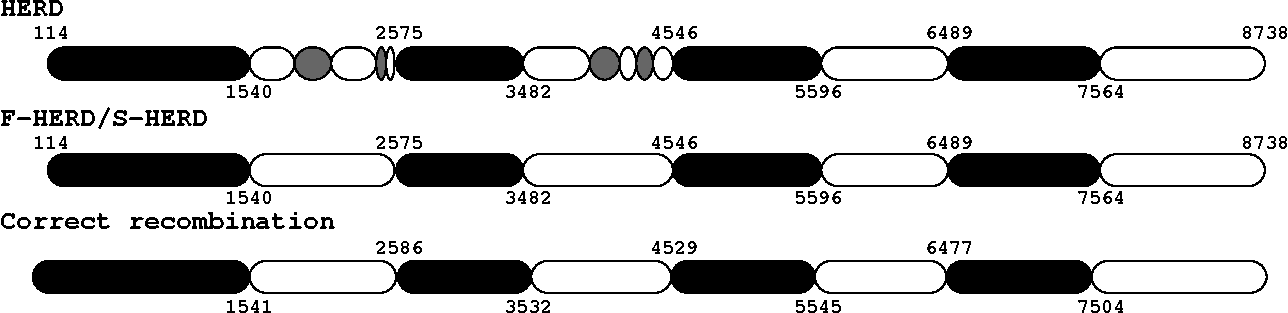
\includegraphics[width=14cm]{../figures/jcss/happyStory.pdf}
\end{center}
\caption[Example of annotation with systematic error.]{ 
Each row corresponds to one annotation of the same HIV recombinant, colors
represents original virus subtypes. Unaltered HERD algorithm predicts wrong
subtype and also contains too many segments. But restricting to the specified
footprint (F-HERD) or to the specified set (S-HERD) provides almost correct
annotation without these errors.  }\label{FIGURE:HERD_BAD} 
\end{figure}

\section{Formal definition}

\begin{note}
In following text, all of the definitions could be done similarly for the
annotations and state paths. Annotations are more general, because by setting
$\lambda$ to identity function, all annotations became state paths.
\end{note}
\todo{Restriction->Guide}

\begin{definition}[Annotation set]
The \abbreviation{\firstUseOf{Annotation set}}{S} of labeling
$\Lambda$ of state path $\pi$ the set of labels visited on the state path.
Let $\pi = \pi_1\pi_2\dots \pi_n$ and $\lambda$ be coloring function as in definition
\ref{DEFINITION:ANNOTATION}. Then 
\[S(\pi) = \left\{\lambda(\pi_1), \lambda(\pi_2)\dots\lambda(\pi_n)\right\}\]

Similarly, since $\Lambda = \Lambda_1\Lambda_2\dots \Lambda_n$ where $\Lambda_i
= \lambda(\pi_i)$, 
\[S(\Lambda) =
\left\{\Lambda_1,\Lambda_2,\dots\Lambda_n\right\}\]

The \firstUseOf{State set} is annotation set where labeling function is identity
function.\label{DEFINITION:ANNOTATION_SET}
\end{definition}

The footprint is what is left from labeling after removing consecutive identical
labels. Formally it was defined in section \ref{SECTION:DISTANTMEASURES} by
definition \ref{DEFINITION::FOOTPRINT}.  We denote the footprint of annotation
$\Lambda$ as $F(\Lambda)$.

Two-stage decoding system can be described in Highest Expected Gain framework
introduced in section \ref{SECTION:HEG}. At first, we define guide and guide
function.

\begin{definition}[Guide function, guide relation, guide]
Let $H$ be an HMM, $f$ be a annotation gain function as in definition
\ref{DEFINITION:GAINFUNCTION} in section \ref{SECTION:HEG}, $L$ be the set of
all annotations, $W$ be an arbitrary set. We call any function
$R:L\to W$ a \firstUseOf{guide function} and $R(\Lambda)$ is
\firstUseOf{guide} $r$ of annotation $\Lambda$.

\firstUseOf{Guide relation} is relation $\hat{R}\subseteq L\times W$
with property that for all $\Lambda\in L$, $(\Lambda, R(\Lambda))\in \hat{R}$.

Similarly to definition of annotation (definition \ref{DEFINITION:ANNOTATION}),
we can define the probability of guide given sequence $X$:

\begin{equation}
\prob{r\mid X, H} = \sum_{\Lambda \in L, R(\Lambda)=r} \prob{\Lambda\mid X, H}
\end{equation}

\end{definition}

Natural way of defining guide relation is following: $(\Lambda, r)\in \hat{R}$
if and only if $R(\Lambda)=R$. However, in some cases it might be useful
to relax the restriction provided by the guide. 

Note that we can see a guide as generalization of annotation. On the other hand,
our use of guides is quite different from our use of annotations. While
annotations are the final product, purpose of guides is to capture some
important properties of the input, that can be subsequently used to find correct
annotation. Finally, we can formally define two-stage decoding:

\begin{definition}[Two-stage decoding]
Let $H$ be an HMM, $f$ be an annotation gain function, $R$ be an guide 
function and $W$ set of all possible guides. Let $X$ be an sequence of
interest and $L$ be the set of all annotations of $X$. In \firstUseOf{two-stage
decoding} we search for annotation $\Lambda$, defined as:

\begin{equation}
\Lambda = \arg\max_{\Lambda'\in L, (\Lambda', r)\in \hat{R}}E_{\Lambda_X\mid
X,H}[f(\Lambda_X,\Lambda')]\label{EQUATION:HIGHEST_EXPECTED_RESTRICTED_REWARD}
\end{equation}
where guide $r$ is defined as
\begin{equation}
r = \arg\max_{r'\in W}\prob{r'\mid H, X}
\label{EQUATION:MOST_PROBABLE_RESTRICTION}
\end{equation}
\end{definition}

Finding the most probable guide can be decoupled from finding the
annotation with highest expected reward. In this chapter we will focus
mainly on the complexity of the first step: finding the most
probable guide. Complexity of the second step, namely finding the annotation
with highest expected gain without guides we studied in \cite{Nanasi2010mgr,
Nanasi2010}. Implementing search with guides is straightforward and we will
discuss it later.

Note that we could use different method to select guide $r$. While it is
possible to use gain functions for defining optimization criteria to select
guide (and altering the equation \ref{EQUATION:MOST_PROBABLE_RESTRICTION}), 
we did not study such variations.

At first we show experiment illustrating effects of the two-stage decoding on
the HIV recombination detection problem.  Further in this chapter we prove that
finding the most probable guide is for certain guide functions NP-hard.

\section{Experiments}

In section \ref{SECTION:HERD} we described HERD decoding. It was used with
jumping HMMs \cite{Schultz2006} for detecting recombinations in HIV virus.
However, using this criteria lead to two artefacts: \begin{itemize} \item
Producing annotations with many short recombinations.  \item Producing
recombinations of wrong virus subtype.  \end{itemize} Example of both type of
errors are illustrated in figure \ref{FIGURE:HERD_BAD} at page
\pageref{FIGURE:HERD_BAD}.

\subsection{Application Domain}
% Az na citacie, toto sa da povazovat za viac menej hotove
\todo{pridaj citacie}
We use problem of recombination detection in HIV virus for the demonstration of
usefulness of two-stage decoding.  This section contains background information
about data used in the experiment.

\begin{figure}
\begin{center}
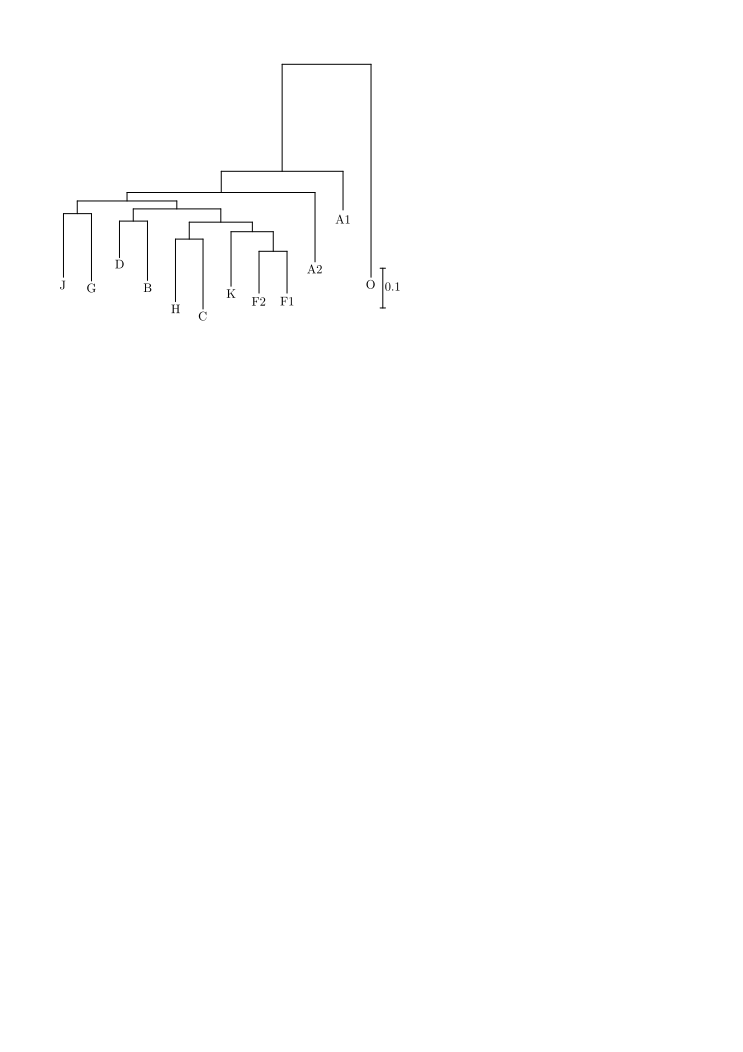
\includegraphics{../figures/hiv_M1strom}
\end{center}
\caption[Phylogenetic tree of the HIV-M1 group]{Phylogenetic tree of the HIV-M1
group of genomes with branch of HIV-O group generated by phyml \cite{Guidon2003}
from database distributed with jpHMM \cite{Schultz2006}. Figure was originally
used in \cite{Nanasi2010mgr}. The lengths of the branches corresponds to the
evolution distances.  }\label{app:figure:phil}
\end{figure}

RNA of HIV virus is sequence roughly $9000$ bases long. Mutation rate of an HIV
virus is high\cite{}, and additionally HIV virus is categorized into several
\firstUseOf{subtypes}\cite{} based on sequence similarity. Phylogenetic tree of
subtypes is show in figure \ref{app:figure:phil}.  Subtypes A and F are further
divided into \firstUseOf{sub-subtypes} A1, A2 and F1, F2.  Due to high sequence
similarity, subtypes B and D are sometimes recognized as sub-subtypes of subtype
BD \cite{}.

Additionally to high mutation rate, \firstUseOf{recombination} occurs in
evolution of HIV virus \cite{}. When recombination occurs, resulting virus is
mosaic combination of two source viruses: recombination of source viruses $v_1$
and $v_2$ is a virus which parts contain sequences from both $v_1$ and $v_2$.  The
position of parts of sequences are retained, so the parts from some region of
recombinant virus is always from the same region in the source virus.
There can be multiple recombination points within same virus and since
recombination can occur between two recombinants, there can be multiple source
subtypes or sub-subtypes in one recombinant. 

Given a recombinant sequence $X$, goal of recombination detection is to label
each base $x$ of sequence $X$ with the subtype from which $x$ originates.  Set
of annotation symbols therefore contain all subtypes/sub-subtypes of HIV virus.
In following text we will use term \firstUseOf{segment}, which is maximal
single-colored consecutive subsequence of annotation.

\subsection{Methods}
\label{HERD:METHODS}
To detect detect recombinations, we have previously used Highest Expected Reward
Decoding \cite{Nanasi2010mgr, Nanasi2010} with same HMM as {\it Schultz et al.
(2006)}\nocite{Schultz2006} used with the Viterbi algorithm. This model and also
their program is called \abbreviation{jumping HMM}{jpHMM} and it a set of
\abbreviation{profile Hidden Markov Models}{profile HMMs}\cite{Durbin1998}
connected with transitions allowing to "jump" between different profiles which
is how the recombination are modeled.

\begin{figure}
\begin{center}
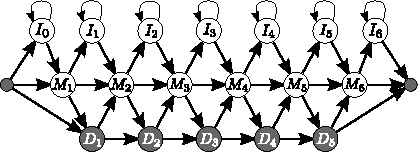
\includegraphics[width=10cm]{../figures/profile_hmm}
\end{center}
\caption[Profile HMM]{Example of profile HMM if length $6$. Shaded states are
silent, the leftmost shaded state is init state. End state is the rightmost
shaded state. Figure is from \cite{Nanasi2010mgr}.}\label{FIGURE:PROFILEHMM}
\end{figure}

Profile HMMs are HMMs with special topology used for matching certain
motifs\cite{Durbin1998}. Profile HMM of length $n$ It consists of match states
$M_1,M_2,\dots, M_n$, insert states $I_0, I_1, \dots, I_n$, silent delete states
$D_1, D_2,\dots, D_n$ and silent init state and silent end state. All states are
connected by transitions as in the figure \ref{FIGURE:PROFILEHMM}. Motif is
represented by chain of match states, each with it's own emission distribution.
Insert states models (short) insertions into the motif. Delete state allows to
skip some parts of the motif. Profile HMMs can be obtained from alignments of
similar sequences and match states would represent the columns of the alignment.
Not all of the columns correspond to match states, columns that
contains gaps above some threshold are usually omitted \cite{Durbin1998}. 

Jumping HMMs are built upon profile HMMs. We start with alignment of all HIV
sequences and construct profile HMM for each subtype or sub-subtype (it depends
whether we want to distinguish between sub-subtypes). We then add global init
state and global end state to connect profiles in parallel.  Column numbers of
each match, insert, and delete states are preserved, so we know the
corresponding column for each states. Additional transitions between different
profiles are added to model recombinations: These "jump" transitions are added
so that they end in the states that corresponds to the nearest following column
of original alignment. Jump from column $c_1$ in subtype $A$ to column $c_2>c_1$
in subtype $B$ is allowed if and only if there is not state in profile of $A$ or
$B$ corresponding to column between $c_1$ and $c_2$. Simplified topology of
jpHMM is in figure \ref{app:fig:jpHMM}. More details can be found in
\cite{Schultz2006, Nanasi2010mgr, Nanasi2010}.

\begin{figure}
\begin{center}
\includegraphics[width=10cm]{../figures/jumping_hmm}
\end{center}
\caption[Jumping HMM]{The simplified structure of jpHMM. Insert and delete state
are omitted from the figure for readability. Picture is taken from our previous
work \cite{Nanasi2010mgr}}\label{app:fig:jpHMM}
\end{figure}

We denote HERD's gain function, described in section \ref{SECTION:HERD}, as
$f_{HERD}$.  Details of algorithm that optimizes this gain function can be found
in \cite{Nanasi2010, Nanasi2010mgr}. In this text we describe modification to
this algorithm so that it can cope with guides. We use the footprint and the
annotation set as a guide functions. In case of footprint we use the natural way
to define guide relation, however in case of the annotation set we use guide
relation $\hat{R}_S$ defined as follows: \[(\Lambda, r)\in
\hat{R}_S\Leftrightarrow R(\Lambda)\subseteq r\]

Original HERD algorithm can be decomposed into two
phases. In the first phase, it constructs \firstUseOf{annotation graph}.
Annotation graph is graph in which each path from the start vertex to the end
vertex represents annotation. Length of such path equals to the expected gain of
corresponding annotation. The longest path in annotation graph therefore
corresponds to the annotation with the highest expected gain. Annotation graph
is directed and acyclic and it's structure is described in figure
\ref{HERD:figure:annotation_graph}.  The second phase consists from finding the
longest path in this graph and converting it to the annotation. Since annotation
graph is directed and acyclic, it is possible to find such path in polynomial
time \cite{Nanasi2010mgr}.

To add guides, we need to change the second phase of the algorithm. We will be
searching for an annotation restricted to the guide with the highest expected
gain. If guide function is annotation set,  we simply remove vertices with
colors that are not in annotation set from the annotation graph and use original
algorithm described in \cite{Nanasi2010mgr}. Since trimming the annotation graph
can be done trivially in linear time, this does not change the computational
complexity of the HERD algorithm.

\begin{figure}
\begin{center}
\includegraphics{../figures/herd_graph}
\end{center} 
\caption[Annotation graph]{Part of a path in an annotation graph with
corresponding annotation. A node with color $c$ and caption $(b,w)$ represents
the vertex $(b,c,w)$ of the graph. The dashed lines connect each vertex to its
corresponding feature. $(b, c, w)$ corresponds to the beginning of $c$-colored
annotation segment starting at position $b$. End of such segment is determined
by the following vertex in path, therefore each edge in the graph correspond to
possible annotation segment. Length of an edge is the expected gain of
corresponding annotation segment. If $w$ is less than maximal window width $W$,
which is parameter of HERD algorithm, the edges from such vertex are allowed
only to vertices of form $(b+w, *, *)$ where $*$ can be any valid value. If
$w=W$, then following edges are of form $(b+W+k, *, *)$ where $k\leq0$.  Figure is
from our previous work \cite{Nanasi2010mgr}}\label{HERD:figure:annotation_graph} 
\end{figure}

Using the footprint as guide requires more changes to the algorithm then just
remove vertices with colors that are not in footprint. To find the longest path,
we have to alter dynamic programming formula for computing the longest path.
We order vertices of annotation graph topologically from start to end vertex
into sequence $v_0, v_2, \dots v_{n-1}$ where $n$ is the number of vertices in
the annotation graph, $v_0$ is the init vertex and $v_{n-1}$ is the end vertex.
This will be the order in which the dynamic programming equations will be
computed.
Let $f=f_0f_2\dots f_{k-1}$ be the footprint we use as a guide and $V[i, j]$ be the length
of the longest path ending in $v_i$ that have footprint $f[:j]$.  Therefore the
length of the longest path with footprint $f$ is $V[n - 1, k]$. If $E$ is the set of
all edges and $C(v_i, v_j)$ is the weight of an edge $(v_i, v_j)$, then $V[i,
j]$ can be computed by following equations: 
\begin{align} V[0, 0] &= 0 \\ V[0, j] &= -\infty, 0< j \leq k \\ V[i, j] &=
\max_{i', (v_{i'}, v_i)\in E} \begin{cases} C(v_i', v_i) + V[i', j]& \text{if
$\lambda(v_i) == \lambda(v_{i'})$}\\ C(v_i', v_i) + V[i', j-1]& \text{if
$\lambda(v_i) \not= \lambda(v_{i'})$ and $\lambda(v_{i'})=f_{j-1}$}\\ 0 &
\text{otherwise} \end{cases} \end{align}

Note that since we have ordered vertices topologically, to compute $V[i, j]$ we
use only values of $V[i', j']$ where $i'< i, j'\leq j$. Therefore we can compute
$V$ with $i$ in increasing order. The longest path can be computed using
back-tracing as in section \ref{SECTION:NEEDLE}. The time and memory complexity 
of this part of the algorithm increased by the factor of $k$. Therefore the time
complexity increases to $O(mWC|E|+mkC^2W^2)$ where $C$ is the number of colors
(labels), $W$ is the window size, $m$ is the length of the sequence and $|E|$ is
the number of transitions in HMM.  Space requirements increased to
$O(\sqrt{m}Cn+WCnk+mkC^2)$. Implementation details of other parts of an
algorithm can be found in \cite{Nanasi2010mgr}.

\subsection{Data \& results}
We created artificial dataset of recombinant HIV sequences and run HERD with two
guide functions: annotation set and footprint. HERD was run with default
parameters, $\gamma=0.2, W=10$. Model was trained using jpHMM program and
alignment of HIV sequences distributed with jpHMM \cite{Schultz2006}.  $10\%$ of
sequences from this alignment were removed from training data and were used for
evaluation. We refer to alignment distributed with jpHMM as \firstUseOf{source
alignment}.

These artificial sequences were generated by alternating segments of two real
sequences from different subtypes. Data were generated from pairwise alignment
of original sequences: if segment $x$ of sequence $X$ follows segment $y$ of
sequence $Y$, then $y$ is immediately after $x$ in the pairwise alignment. We
did experiments with two types of segment lengths: either $200-300$ (short) or
$950-1050$ (long) with additional $0-750$ and $0-500$ bases for the first and
for the last segment respectively. Length of each segment was drawn from uniform
distribution.  Pairwise alignments were obtained from source alignment of HIV
sequences.

\todo{Tieto experimenty by som radsej zbehol este raz}
Apart from two different recombination length, we also evaluated algorithm of
recombinants of sequences from same subtypes but different sub-subtypes, which
gave us $4$ different data sets. For all datasets we generated $150$
recombinants of two sequences. For subtypes we use subtypes A, BD, C, F, G. For
sub-subtypes we . For sub-subtypes we have used sub-subtype pairs A1-A2, B-D and
F1-F2.

Since finding the most probable set or the most probable footprint is con
tractable, we used approximations in this experiments. The approximations of the
most probable set and the most probable footprint for given recombinant were
taken from program balls by \cite{Brown2010}, which is also described in section
\ref{SECTION:DISTANTMEASURES}. Note that balls algorithm estimate footprint by
sampling of the state paths. For using set as guide, we have chosen to take the
set of labels used in footprint as an approximation to the most probable set,
since these sets were almost always correct. Note that the aim of these
experiments is to demonstrate the usefulness of two-stage decoding approach, not
to compare it with the other methods for recombination detection.

To measure performance of the algorithm and amount of systematic errors, we use
following metrics to compare different versions of algorithm.
\begin{enumerate}
\item {\bf \%id}: Percentage of the bases with correctly predicted label.

\item {\bf Segment specificity}: Percentage of the number of correctly predicted
segments out of the number of all predicted segments. Segment is correctly
predicted if it's boundaries are within $10$ bases.

\item {\bf Segment sensitivity}: Percentage of the number of correctly predicted
segments out of the number of segments in the correct alignment.

\item {\bf \%correct footprints}: Percentage of correctly predicted footprints.

\item {\bf Footprint distance}: Normalized edit distance of predicted footprint
and correct footprint (averaged over all samples).

\item {\bf Set specificity}: Percentage of the number or correctly predicted label
types out of the total number of predicted labels.

\item {\bf Set sensitivity}: Percentage of the number of correctly predicted label
types out of the total number of label types in correct labeling.

\end{enumerate} 
Aim of measures $1-3$ is to quantify the performance of the algorithm in terms
of ability to correctly predict the correct annotation. Measures $4-7$ quantify
the amount of previously mentioned systematic errors in predicted annotation.

We use three versions of HERD in our experiments: original version of HERD,
version with annotation set as a guide denoted by S-HERD and version using
footprint as a guide denoted by F-HERD. The results of experiments are in the
table \ref{HERD:EXPTABLE}. 

\begin{table*}
\begin{center}
\begin{tabular}{cccccccc}\hline
&{\bf \%id}&\bf segment&\bf segment&\bf \%correct&\bf footprint&\bf set&\bf  set\\ 
&&\bf sp.& \bf sn.& \bf footprints&\bf distance&\bf    sp.&\bf  sn.\\ 
\hline
\hline
\multicolumn{8}{l}{\bf subtypes, short recombination length}\\
HERD   &88.09& 65.59& {\bf 67.71}& 30.67& {\bf 0.0376}& 56.7&{\bf 100}\\
S-HERD &{\bf 88.55}& {\bf 68.17}& {\bf 67.71}& {\bf 37.33}& 0.0380& {\bf 99.3}&{\bf 100}\\
F-HERD &84.71& 65.02& 58.19& 2.67& 0.0928& {\bf 99.3}&{\bf 100}\\\hline
\multicolumn{8}{l}{\bf sub-subtypes, short recombination length}\\
HERD   &{\bf 72.72}& 32.79& {\bf 27.56}& {\bf 0.0}&    {\bf 0.2083}& 19.3&{\bf 100}\\
S-HERD &72.33&{\bf 35.77}& 26.59& {\bf 0.0}&    0.2656& {\bf 100}&{\bf 100}\\
F-HERD &68.05&30.65& 16.97& {\bf 0.0}&    0.3228& {\bf 100}&{\bf 100}\\\hline
\multicolumn{8}{l}{\bf subtypes, long recombination length}\\
HERD   &93.86& 50.20& 61.82& 76.67& 0.0246& 77.3&{\bf 100}\\
S-HERD &94.12& 53.46& 63.68& 98.67& 0.0015&   {\bf 100}&{\bf 100}\\
F-HERD &{\bf 94.19}& {\bf 53.57}& {\bf 63.83}& {\bf 100}&    {\bf 0.0}&
{\bf 100}&{\bf 100}\\\hline
\multicolumn{8}{l}{\bf sub-subtypes, long recombination length}\\
HERD   &84.10& 19.87& 25.63& 21.33& 0.1491& 29.3&{\bf 100}\\
S-HERD &83.90& 24.87& 28.55& 47.97& 0.0524& {\bf 98.6}&{\bf 100}\\
F-HERD &{\bf 85.03}& {\bf 26.65}& {\bf 30.24}& {\bf 98}&   {\bf 0.0018}& {\bf
98.6}&{\bf 100}\\
\end{tabular}
\end{center}
\caption[Results of F/S-HERD on artificial recombinants.]{Results of experiments
on four data sets. Larger values are better for all columns  except
{\it footprint distance} column where lower value is better. Best value out of
each column is bold.}\label{HERD:EXPTABLE}
\end{table*}

In general, we expect short recombination length to be harder than long
recombination length and additionally distinguishing between sub-subtypes is
harder than distinguishing between subtypes. Both of these expectations were
observed in the results. In all experiments on recombinants with long
recombination length, F-HERD outperformed HERD in all metrics, especially with
the metrics $4-7$: percent of correct footprint was increased from $76.67\%$ to
$100\%$ in case of subtypes and from $21.33\%$ to $98\%$ in case of
sub-subtypes. However on recombinants with short recombination length,
footprints used were wrong most of the time and in sub-subtypes dataset all of
the algorithms predict zero correct footprints.  In fact, performance of F-HERD
decreased in all metrics but annotation set specificity and sensitivity. This
and increase in footprint distance suggests that improvement in finding the best
footprint is needed.


S-HERD performs slightly worse than F-HERD on the long recombination length, but
the metrics were still significantly better than unguided HERD algorithm.
Additionally, using S-HERD with short recombination length was not performing
worse then HERD, but their performance was similar.

\section{Computational complexity problems}

In the previous experiments, we demonstrated that two-stage algorithm can be
useful technique to improve decoding algorithm. In this and following sections
we will discuss mostly theoretical aspects of defining guides and finding the
most probable guides. In particular, we show that following problems are
NP-hard: \firstUseOf{the most probable set},
\firstUseOf{the most probable footprint}, and \firstUseOf{the most probable
restriction}. The last problem is variant of the most probable set.


\begin{definition}[The most probable set problem] Given an HMM $H$, sequence $X$ of
length $n$ and a number $p\in [0,1]$, decide if there exists a set of states $S$
such that $\prob{S(\pi) = S, X\mid H} \geq p$.
\end{definition}

\begin{theorem}
The most probable set problem is NP-hard. \label{THEOREM::NPSET}
\end{theorem}

In the most probable set problem, guide restricts us only to paths that use all
of the states from annotation set. As in the experiments, it is more natural to 
allow also to use only subsets of annotation set in the alignment. Therefore we
might be interested in maximizing $\prob{S(\pi) \subseteq S, X\mid H}$. However, 
in this case we would get the set of all labels. To get a meaningful and useful
problem definition, we can restrict the size of an annotation set to be $k$:

\begin{definition}[The most probable restriction problem]
Given an HMM $H$, sequence $X$, integer $k$ and number $p\in[0,1]$, decide if
there exists a subset of states $S$ of size $k$, such that
$\prob{S(\pi)\subseteq S, X\mid H} \geq p$.
\end{definition}

\begin{theorem}
The most probable restriction problem is NP-hard. \label{THEOREM::NPREST}
\end{theorem}

Finally, we also show that the most probable footprint problem is NP-complete.
\begin{definition}[The most probable footprint problem]
Given an HMM $H$, sequence $X$
of length $n$ and a number $p\in [0,1]$, decide if there exists a footprint $F$
such that $\prob{f(\pi) = S, X\mid H}\geq p$
\end{definition}

\begin{theorem}
The most probable footprint problem is NP-complete.
\label{THEOREM::NPFOOT}
\end{theorem}


At first we show combinatorial proof of theorem \ref{THEOREM::NPSET}. Then we
show proof of theorem \ref{THEOREM::NPREST}. Finally we show proof of theorem
\ref{THEOREM::NPFOOT} by showing $8$-state HMM for which is NP hard to find the
most probable footprint and then we extend this prove theorem
\ref{THEOREM::NPSET} again. 

\section{The Most Probable Set Problem}
\label{sec:set}

\begin{definition*}[The most probable set problem] Given an HMM $H$, sequence $X$ of
length $n$ and a number $p\in [0,1]$, decide if there exists a set of states $S$
such that $\prob{S(\pi) = S, X\mid H} \geq p$.
\end{definition*}

In this section, we prove NP-hardness of the most probable set problem, theorem \ref{THEOREM::NPSET}.

\begin{comment}
\begin{theorem}The following problem is NP-hard:
Given an HMM $H$, sequence $X$ of length $n$, and a number $p\in [0,1]$,
decide if there exists a set of states $S$ such that 
$\Pr\left(s(\pi)=S, X\mid H, n \right)\geq p$.
\end{theorem}\label{thm:sets}
\end{comment}

\todo{Vloz sem definiciu max clique, alebo aspon cituj}
To prove this theorem, we will use a reduction from the maximum clique
problem.  Given a graph $G=(V,E)$ and a clique
size $k$, we first choose a suitable threshold $k'\ge k$, as
detailed below, and construct a graph $G'=(V',E')$ such that $G'$ has
a clique of size $k'$ if and only if $G$ has a clique of size
$k$. This is achieved simply by adding $k'-k$ new vertices and
connecting each of the new vertices to all other vertices in $V'$.
As long as $k'-k$ is not too large, this transformation can be done in
polynomial time.

In the next step, we use $G'$ and $k'$ to construct an HMM $H_{G'}$, an input
sequence and a probability threshold. $H_{G'}$ have property the set with
probability above threshold on given sequence corresponds to the clique of size
$k'$ in graph $G'$. We will use the following
straightforward way of converting a graph to an HMM.

\begin{definition}\label{GraphHMM}
Let $G=(V,E)$ be an undirected graph (without self-loops). 
Then the \emph{graph HMM} $H_G$ is defined as follows:
\begin{itemize}
\item Its set of states is $V\cup \{\psi\}$, where $\psi\notin V$ is a
  new state called the error state.
\item Its emission alphabet is $\{0,1\}$.
\item Each state $v\in V$ has initial probability $I_{v} = 1/|V|$, the
error state has initial probability $I_{\psi}=0$.
\item Each state $v\in V$ emits 0 with probability 1, the error state emits 1 
with probability 1.
\item Transitions with non-zero probability between states $u,v\in V$
  correspond to edges in $E$:
$$a_{u,v}=\begin{cases}
\frac1{|V|} & \{u,v\}\in E\\
0 & \text{otherwise}
\end{cases}$$
\item $a_{u,\psi}=1-\sum_{v\in V}a_{u,v}$
and $a_{\psi,u}=0$ for all $u\in V$. The error state has a self-transition with
probability 1: $a_{\psi,\psi}=1$.
\end{itemize}
\end{definition}

The purpose of error state $\psi$ is to level the probabilities of admissible
state paths without $\psi$ to the same probability. Since $\psi$ is the only
states that generates $1$, only sequences of form $X=0^n$ can be generated by
admissible state path. Emission probabilities on such strings are $1$, initial
probability and all transitions are equal to $|V|^{-1}$, and therefore
$\prob{\pi, X=0^n\mid H_G,n} = |V|^{-n}$.  Each such path corresponds to walk in
graph $G$. Each set of states in $H_G$ naturally correspond to subset of states.
The probability of the set is proportional to the number of corresponding walks
in the graph $G$. Therefore we will count the number of special walks in induced
subgraphs of $G$.

\begin{definition}
Let $G=(V, E)$ be a graph and $S\subseteq V$ be arbitrary set of its vertices.
Then walk $w=v_1v_2\dots v_n, v_i\in V$ of length $n-1$ \firstUseOf{cover} set
$S$, if and only if $\left\{v_1, v_2, \dots, v_n\mid 1\leq i\leq n\right\}=S$. 
We say that walk $w$ cover graph $G$ if $w$ cover graphs set of vertices $V$.

In other words, walk cover set $S$ if it uses only vertices from $S$ and each
vertex from $S$ is used at least once.
\end{definition}

Let $Y(n, G)$ be the number of graph covering walks of length $n-1$. Since walk
of length $n - 1$ contain $n$ vertices, $Y(n, G)=0$ if $n<|V|$. We consider a
special case of this formula for complete graphs: Let $K_k$ be
complete graph with $k$ vertices, then $D(n, k) = Y(n, K_k)$. Following claim
clearly holds:

\begin{lemma}\label{NotCliqueIsSmaller}
If $G$ is a graph with $k$ vertices and $n\ge k$, then
$Y(n,G)\le D(n,k)$ with equality only for $G=K_k$. 
\end{lemma}

In our reduction, we use HMM $H=H_{G'}$ and $X=0^n$ for a suitable choice of $n$
discussed below. We will set threshold $p$ to $D(n,k')/|V|^{n}$. Clearly, if the
input graph $G$ has a clique $S$ of size $k$, graph $G'$ has a clique $S'$ of
size $k'$. There are $D(n,k')$ walks of length $n-1$ that cover $S'$. Each such
walk corresponds to one state path, and therefore the probability of the set of
states $S'$ is exactly $p$. 

In order to prove the opposite implication "if there exists a state path with
probability $p$ then there is clique of size $k$ in graph", we need suitable choices
of $n$ and $k'$. Table \ref{DNKTable} shows values of $D(n,k)$ for
small values of $n$ and $k$. For a fixed length of walk $n$, the
number of walks in $K_k$ initially grows with increasing $k$, as we
have more choices which vertex to use next, but as $k$ approaches $n$,
$D(n,k)$  may start to decrease, because the walks are more constrained by
the requirement to cover every vertex. We are particularly interested in
the value of $k$ where $D(n,k)$ achieves the maximum value for a fixed $n$. 
In particular we use the following notation:
$$M_{n} = \min\left\{k ; D(n,k) = \max_{0\leq k'\leq
  n}D(n,k')\right\}$$
  
Note that if there are multiple values
of $k$ achieving maximum, we take the smallest one as $M_n$.  In our
reduction, we would like to set $n$ to be the smallest value such that
$M_n=k$, but we were not able to prove that such $n$ exists for each $k$.
Therefore we choose as $n$ the smallest value such that $M_n\ge k$, and 
we denote this value $n_k$. As $k'$ we then use $M_{n_k}$. The following 
lemma states important properties of $n_k$ and $M_{n_k}$. 

\begin{table*}
\begin{center}
\begin{tabular}{|c||c|c|c|c|c|c|c|c|c||c|}\hline
\bf n/k&\bf 0&\bf 1&\bf 2&\bf 3&\bf 4&\bf 5&\bf 6&\bf 7&\bf 8&\bf
$\mathbf{M_n}$\\\hline\hline
\bf 0&{\bf 1}&&&&&&&&&0\\\hline
\bf 1&&\bf 1&&&&&&&&1\\\hline
\bf 2&&&\bf 2&&&&&&&2\\\hline
\bf 3&&&2&\bf 6&&&&&&3\\\hline
\bf 4&&&2&18&\bf 24&&&&&4\\\hline
\bf 5&&&2&42&\bf 144&120&&&&4\\\hline
\bf 6&&&2&90&600&\bf 1200&720&&&5\\\hline
\bf 7&&&2&186&2160&7800&\bf 10800&5040&&6\\\hline
\bf 8&&&2&378&7224&42000&100800&\bf 105840&40320&7\\\hline
\bf 9&&&2&762&23184&204120&756000&\bf 1340640&1128960&7\\\hline
\bf 10&&&2&1530&72600&932400&5004720&13335840&\bf 18627840&8\\
\hline\hline
$\mathbf{n_k}$&0&1&2&3&4&6&7&8&10&\\\hline 
$\mathbf{M_{n_k}}$&0&1&2&3&4&5&6&7&8&\\\hline 
\end{tabular}
\end{center}
\caption{Values of $D(n,k)$, $n_k$, $M_n$, and $M_{n_k}$ for small values of $n$ and $k$. Empty cells contain zeros.}\label{DNKTable}
\end{table*}

\begin{lemma}\label{LEMMA:DNKlemma}
The value of $n_k$ is at most $\lceil k\ln k\rceil$, and $n_k$ and
$M_{n_k}$ can be computed in polynomial time.
\end{lemma}

Before proving this lemma, we finish the proof of the reduction. Let
us assume that there is a set of states $S$ such that
$\prob{s(\pi)=S,X \mid H,n}\ge p$. This means that if we consider walks in the
subgraph $G'(S)$ induced by the set $S$, we get $Y(n,G'(S))\ge
D(n,k')$. We will consider three cases:
\begin{itemize}
\item If $S$ is a clique and $|S|\ge k'$, we have the desired clique in 
graph $G'$, and therefore there is also a clique of size $k$ in graph $G$. 
\item If $S$ is a clique and $|S|<k'$, then by definition of $M_n$ we have 
$Y(n,G'(S))=D(n,|S|)<D(n,M_n) = 
D(n,k')$. This is a contradiction with our assumption. 
\item If $S$ is not a clique, then by Lemma \ref{NotCliqueIsSmaller}
  and definition of $M_n$ we have $Y(n,G'(S)) < D(n, K_{|S|}) \le
  D(n,M_n) = D(n,k')$. Again we get a contradiction with 
the inequality $Y(n,G'(S))\ge D(n,k')$.
\end{itemize}
Therefore, we have proved that $G$ contains a clique of size $k$ if and
only if the most probable set of states in $H_{G'}$ that can generate $X$ has
probability at least $p$. Moreover, we can construct $n_k$, $M_{n_k}$,
$H_{G'}$, $X$, and $p$ in polynomial time.
To complete this proof we need to prove Lemma \ref{LEMMA:DNKlemma}.  We
start by proving another useful lemma.

\begin{lemma}\label{RecurenceLemma}
The following recurrence holds for $2\leq k\leq n$:
$$D(n,k)=(k-1) D(n-1,k) + k D(n-1,k-1).$$
In addition, $D(n,n)=n!$, $D(n,1) = 0$ for $n>1$, and $D(n,k) = 0$ for $k>n$.
\end{lemma}

\begin{reformulate*}
Chcem sem este pridat text ako sa to podoba a suvisi s tymi eulerovymi vecami.
Ale musim to znova najst.
\end{reformulate*}

\begin{proof}
Clearly, $D(n,n)=n!$ since walks of length $n-1$ correspond to
permutations of vertices.  If $n>1$ then $D(n,1)=0$, since $K_1$ does
not contain any edges.  If $k>n$, $D(n,k)=0$ since a walk of length
$n-1$ can pass through at most $n$ vertices.

Now let $2\leq k\leq n$. Denote as $v(w)$ the number of different
vertices covered by walk $w$. Let $w$ be a walk of length $n-1$ with
$v(w)=k$ and let $w'$ be a walk obtained by taking the first 
$n-1$ vertices of walk $w$. Then $v(w')$ is either $k$ or $k-1$. 

Every walk $w'$ of length $n-2$ with $v(w')=k$ can be extended to a
walk $w$ of length $n-1$ in $K_k$ in $k-1$ ways, because as the last vertex
of $w$ we can use any vertex except the last vertex of $w'$. Therefore
there are $(k-1) D(n-1,k)$ different walks $w$ in $K_k$ with
property $v(w')=k$.

On the other hand if $v(w')=k-1$, we can create a walk $w''$ in
$K_{k-1}$ by renumbering the vertices in $w'$ so that only numbers
$\{1,\dots,k-1\}$ are used (if the vertex missing in $w'$ is $i$, we
replace $j$ by $j-1$ for every vertex $j>i$).  The same
representative $w''$ is shared by $k$ different walks $w$, because to
create $w$ from $w''$, we need to choose the missing vertex $i$ from
all $k$ possibilities, renumber vertices to get $w'$ and then to add
the missing vertex $i$ at the end of the walk. Therefore there are
$kD(n-1,k-1)$ walks with the property $v(w')=k-1$. Combining the two
cases we get the desired recurrence.\qed
\end{proof}

\begin{proof}[Proof of Lemma \ref{LEMMA:DNKlemma}] 
Assume that $k\ge 3$. Clearly, $D(n,k)\leq k(k-1)^{n-1}$, since
$k(k-1)^{n-1}$ is the number of all walks of length $n-1$ in
$K_k$. However, this number includes also walks avoiding some
vertices. The number of such walks can be bounded from above by
$k(k-1)(k-2)^{n-1}$ where we choose one of the $k$ vertices to avoid
and then consider all possible walks on the remaining $k-1$
vertices. In this way we count some walks multiple times; nonetheless
by Bonferroni inequality we obtain bound $$D(n,k)\geq
k(k-1)^{n-1}-k(k-1)(k-2)^{n-1}$$

For $k\ge 4$ we therefore have that if
$$(k-1)(k-2)^{n-1}<k(k-1)^{n-1}-k(k-1)(k-2)^{n-1}$$, then
$D(n,k-1)<D(n,k)$.  By taking logarithm of both sides of the inequality, we
obtain $n>f(k)$ where $$f(k) = 1+\frac{\ln(k^2-1)-\ln
  k}{\ln(k-1)-\ln(k-2)}$$  Let $n = \lceil f(k)\rceil$ for some $k\ge
4$ and consider row $n$ in Table \ref{DNKTable}.
We have that $D(n,k-1)<D(n,k)$ and since function $f$ is
increasing, we also we have that $D(n,k'-1)<D(n,k')$ for all $k'\le k$ 
(we have proved it only for $k'\ge 4$, but it is easy to see that it is
also true for $2\le k'\le 3$). The maximum in row $n$ is therefore
achieved at some position $M_n \ge k$. Recall, that $n_k$ is the
smallest $n$ such that $M_n\ge k$. Therefore $n_k\leq \lceil f(k)\rceil$.
The function $k \ln k/f(k)$ is decreasing and its limit is $1$ as $k$
approaches $\infty$. Therefore $\lceil f(k)\rceil\leq\lceil k\ln k\rceil$,
which gives us the inequality $n_k\le \lceil k \ln k\rceil$. This inequality 
can also be easily verified for $k<4$. Since $M_n\le n$,
we also have $M_{n_k}\le \lceil k \ln k\rceil$. 

We can compute $n_k$ and $M_{n_k}$ by filling in table $D(m,j)$ for
all values of $m$ and $j$ up to $\lceil k\ln k\rceil$ using the
recurrence from Lemma \ref{RecurenceLemma}. Since $D(n,k)\leq k^n\leq
n^n$, we can store $D(m,j)$ in $O(k \mbox{polylog}(k))$ bits.
Therefore computing the desired values $n_k$ and $M_{n_k}$ 
can be done in polynomial time. \qed
\end{proof}

%By using the same reduction as in Theorem \ref{thm:sets}, we can
%also prove NP-hardness of the following variant of the problem, in
%which we restrict the size of the set of states $S$. 

%\begin{corollary}
%The following problem is NP-hard:
%Given is an HMM $H$, sequence
%$X$ of length $n$, integer $k$ and a number $p\in [0,1]$ and the task to
%decide if there exists a set of states $S$ of size exactly $k$ 
%such that $\Pr\left(s(\pi)=S, X\mid H, n \right)\geq p$.
%\end{corollary}

%We can easily see that the existence of a clique
%of size $k$ in $G$ leads to the existence of the desired set of states
%$S$ of size exactly $k'$, and by following the reasoning from the
%proof, we can also prove that the converse is true.

Note that it is not clear if the most probable set of states problem is in
NP. In particular, given a set of states $S$, it is NP-hard to find out if its
probability is greater than some threshold $p$, even if this threshold
is 0, as we show next.

\begin{theorem}
Given HMM $H$, sequence $X$ of length $n$ 
and a subset of state space $S$, the problem of deciding if
$\Pr\left(s(\pi)=S, X\mid H, n\right)$ is non-zero is NP-complete.
\end{theorem}

\begin{proof} Proof is reduction to problem of finding Hamiltonian path.

\begin{definition}\label{GraphHMM}
Let $G=(V,E)$ be an undirected graph (without self-loops). 
Then the \emph{graph HMM} $H_G$ is defined as follows:
\begin{itemize}
\item Its set of states is $V\cup \{\psi\}$, where $\psi\notin V$ is a
   new state called the error state.
\item Its emission alphabet is $\{0,1\}$.
\ item Each state $v\in V$ has initial probability $I_{v} = 1/|V|$, the
error state has initial probability $I_{\psi}=0$.
\item Each state $v\in V$ emits 0 with probability 1, the error state emits 1 
with probability 1.
\item Transitions with non-zero probability between states $u,v\in V$
  correspond to edges in $E$:
$$a_{u,v}=\begin{cases}
\frac1{|V|} & \{u,v\}\in E\\
0 & \text{otherwise}
\end{cases}$$
\item For $u\in V$, we also have $a_{u,\psi}=1-\sum_{v\in V}a_{u,v}$
and $a_{\psi,u}=0$. The error state has a self-transition with 
probability 1: $a_{\psi,\psi}=1$.
\end{itemize}
\end{definition}

The error state $\psi$ is added to the HMM so that all non-zero
transitions between states in $V$ have the same probability. Any state
path $\pi$ containing only states from $V$ connected by transitions
with non-zero probability has the same probability of generating
sequence $X=0^n$: $\Pr(\pi, X=0^n|H_G,n) = |V|^{-n}$.
%Such paths correspond to walks in graph $G$.

Let $G=(V,E)$ be a graph  
and $H_G$ be the corresponding graph HMM as
in Definition \ref{GraphHMM}. Let $X=0^{|V|}$.  
%Any state path
%that can generate $X$ and contains all vertices from $V$ contains each
%vertex exactly once.  
It is easy to see that $\Pr\left(s(\pi)=V,X \mid H_G, |X|
\right)>0$ if and only if $G$ contains a Hamiltonian path. \qed
\end{proof}

The most probable set problem is
fixed-parameter tractable with respect to the size of the HMM. Given
an HMM with $m$ states and a sequence of length $n$, we can find the
most probable set of states in time $O(2^m m^2 n)$ by a dynamic
programming algorithm similar to the Forward algorithm.
We define $F[i,S,v]$ to be the sum of probabilities of all
states paths $\pi$ of length $i$ such that $s(\pi)=S$, $\pi$ ends in
state $v$ and generates the first $i$ characters of sequence $X$.
To compute $F[n,S,v]$, we use the following equation:
\ifx\settwocolumn\undefined
$$F[i,S,v] = \begin{cases}
I_{v}e(v,X[1])& i=1,S=\{v\}\\ 
\displaystyle \sum_{u\to v}a_{u,v}e(v,X[i])\left(F[i-1,S\backslash\{v\},u]
+ F[i-1,S,u]\right) & i>1, v\in S\\
0 & \mbox{otherwise}
\end{cases}$$
\else
$$F[i,S,v] = \begin{cases}
I_{v}e(v,X[1])& i=1,S=\{v\}\\ 
\displaystyle \sum_{u\to v}a_{u,v}e(v,X[i])\\\hspace{5mm}\left(F[i-1,S\backslash\{v\},u]\right.
\\\hspace{5mm}\left.
+ F[i-1,S,u]\right) & i>1, v\in S\\
0 & \mbox{otherwise}
\end{cases}$$
\fi
\section{The Most Probable State Restriction}

\label{sec:restriction}


\begin{definition*}[The most probable restriction problem]
Given an HMM $H$, sequence $X$, integer $k$ and number $p\in[0,1]$, decide if
there exists a subset of states $S$ of size $k$, such that
$\prob{S(\pi)\subseteq S, X\mid H} \geq p$.  
\end{definition*}

In this section we prove that the most probable restriction problem is
NP-complete.
\begin{proof}
We will prove NP-hardness by a reduction from 3-SAT. Consider an
instance of 3-SAT with the set of variables $U=\{u_1,u_2,\dots,u_n\}$
and the set of clauses $C=\{c_1,c_2,\dots,c_m\}$. 
Based on sets $U$ and $C$, we construct an HMM $H$ as
follows.  The set of states $V$ will contain all positive and negative
literals. The emission alphabet $\Sigma$ contains all clauses, all
variables and a special error symbol $\psi$. The initial probability
of each state is $1/(2n)$, and the transition probability
between any two states is also $1/(2n)$. State for a literal
$u$ emits with probability $1/|\Sigma|$ every clause that contains $u$.
State for literal $u$ also generates the positive form of the literal
with probability $1/|\Sigma|$. For proper normalization, 
it also generates the error symbol 
with probability $1-\sum_{x\in C\cup U}e(v,x)$. 

We also create string $X=u_1u_2\dots
u_nc_1c_2\dots c_m$ and set the size of the restriction $k$ to equal
the number of variables $n$. Every state path $\pi$ that can generate
$X$ has probability $(2n|\Sigma|)^{-|X|}$; we set threshold $p$ to
this value. Each 
variable $u_i$ in the first part of $X$ 
can be generated only by states $u_i$ and
$\bar{u_i}$; therefore one of these states needs to be in the
path. The first portion of the path thus traverses $k$ 
different states; only these states can be used to emit the second part of the
sequence. 
%Every clause can be emitted only by states for literals that
%satisfy it. 
The set of states used by a state path with
non-zero probability therefore corresponds to a satisfying assignment
in a straightforward way. 
%The HMM has a restriction of size $k$ with
%probability at least $p$ if and only if the 3-SAT instance has a
%satisfying assignment.

Note that given a restriction $S$, we can easily verify if its
probability is at least $p$ by a variant of the Forward algorithm
in which we allow only states in $S$. Therefore the problem is in NP.
\qed
\end{proof}


\section{The Most probable footprint}
\label{sec:footprint}

\begin{comment}
Finding the most probable
footprint is a reasonable decoding criterion,
and it may also serve as a starting point in a multi-stage
strategy. In this section, we show that this problem is
NP-hard. In particular, we will consider the footprint of a state path
$f(\pi)$. The problem of optimizing the footprint of a labeling
$f(\ell(\pi))$ is also NP-hard, because optimizing $f(\pi)$ is its special case, 
equivalent to optimizing $f(\ell(\pi))$ in an HMM in
which each state has a unique label.
\begin{theorem}
There is a fixed HMM $H$ such that the following problem is NP-complete:
Given a sequence $X$ of length $n$ and probability $p\in [0,1]$, determine
if there is a footprint $F$ such that $\prob{f(\pi)=F,X\mid H,n}\ge p$.
\label{thm:foot}
\end{theorem}
\end{comment}


\begin{figure*}
\centerline{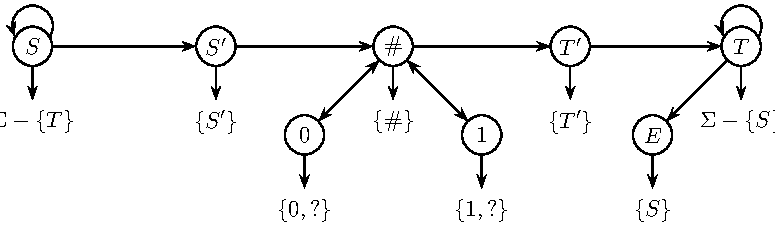
\includegraphics[scale=0.68]{../figures/jcss/cliquehmm.pdf}}
\caption[HMM for which footprint is NP-hard to optimize]{\label{fig:footprint_hmm} The HMM from the proof of Theorem
  \ref{THEOREM::NPFOOT}. States are shown as circles; under each we
  list the set of symbols that the state emits with non-zero
  probability. Each of these symbols is emitted with probability
  $1/k$, where $k$ is the size of the set. The HMM always starts in
  state $S$. All outgoing transitions from a particular state have
  the same probability.}
\end{figure*}

\begin{definition*}[The most probable footprint problem]
 Given an HMM $H$, sequence $X$
of length $n$ and a number $p\in [0,1]$, decide if there exists a footprint $F$
such that $\prob{f(\pi) = S, X\mid H}\geq p$
\end{definition*}

\begin{proof}
We will prove NP-hardness by a reduction from the maximum clique problem
using the HMM in Figure 
\ref{fig:footprint_hmm} with eight states and
alphabet $\Sigma=\{S,S',T,T',\#,0,1,?\}$. 

%Popis zakodovania grafu
Let $G=(V,E)$ be an undirected graph with $n$ vertices $V=\{1,2,\dots,n\}$. We
will encode it in a sequence $X$ over alphabet $\Sigma$ as follows.  For every
vertex $v\in V$, we create a block $X_v$ with $2n+3$ symbols:
$X_v=S'\#b_{v,1}\#b_{v,2}\#\dots\#b_{v,n}\#T'$, where $b_{i,j}=1$ if $i=j$,
$b_{i,j}=?$ if $(i,j)\in E$ and $b_{i,j}=0$ otherwise.  Sequence $X$ is a
concatenation of blocks for all vertices with additional first and last symbols:
$X=SX_1X_2\dots X_nT$.

All state paths that can generate $X$ have a similar structure. The first
symbol $S$ and several initial blocks are generated in state $S$, one
block, say $X_i$, is generated in states $S'$, $\#$, $0$, $1$, and
$T'$ and the rest of the sequence, including the final symbol $T$, is
generated in state $T$. We will say that a state path with this
structure \emph{covers} the block $X_i$.  Note that state $E$ is never used in
generating $X$, its role is to ensure that the probability of
self-transition is the same in states $S$ and $T$.
All state paths that can generate $X$ have the same
probability $q = \Pr(\pi,X\mid H,|X|) = 2^{-2n^2-2n}3^{-n-1}7^{-2n^2-n+1}$.

%celkovo 2n^2+3n+2 symbolov
%1/2 zacni v S
%kazdy symbol v S a T ma 1/7 emisiu a 1/2 tranziciu do dalsieho
% tych symbolov je 2n^2+n-1
%prechody z S' a T', 0, 1 su 1, tych je n+2
%prechody z # so 1/3, tych je n+1
%emisia v S' a T' a # je 1, tych je n+3
%emisia v 0 a 1 je 1/2, tych je n
%
%spolu teda 1/2^{1 + 2n^2+n-1 + n} * 1/3^{n+1} * 1/7^{2n^2+n-1} 


We say that a state path $\pi$ is a \emph{run} of footprint $F$, if
$\pi$ can generate $X$, and $f(\pi)=F$.
Every footprint that can generate $X$ has the following structure:
$F=SS'\#c_1\#c_2\#\dots\#c_n\#T'T$, where $c_i\in\{0,1\}$. 
The probability of footprint $F$ is $qk$, where $k$ is the number of its runs.
Also note that every run of $F$ covers a different $X_i$, because once $X_i$
is known, the whole path is uniquely determined. 

We will now prove that the graph $G$ has a clique of size at least $k$
if and only if there is a footprint for sequence $X$ with
probability at least $qk$.  First, let $R$ be a clique in $G$ of size
at least $k>0$.  Consider the footprint
$F=SS'\#c_1\#c_2\#\dots\#c_n\#T'T$ where $c_i=1$ if $i\in R$ and $c_i=0$
otherwise. For any $i\in R$, there is a run $\pi_i$ of $F$ that covers
$X_i$. This run will use state 1 for generating each $b_{i,j}$ such
that $j\in R$ and thus both $b_{i,j}\in \{?,1\}$ and $c_j=1$.  For
$j\notin R$ we have $b_{i,j}=0$ and $c_j=0$, thus they will use state
0 in $\pi$. Since there is a different run for every $i\in R$, footprint 
$F$ has at least $k$ runs.



Conversely, let $F$ be a footprint with probability at least $qk>0$
and thus with at least $k$ runs. We will construct a clique of size at
least $k$ as follows. Let $R$ be the set of all vertices $i$ such that
$f$ has a run that covers $X_i$. Clearly the size of $R$ is at least
$k$.  Since $F$ has non-zero probability, it has the form
$SS'\#c_1\#c_2\dots\#c_n\#T'T$ for $c_i\in \{0,1\}$. For all $i\in R$,
$c_i=1$ because the $i$-th block has $b_{i,i}=1$. Therefore for all
$i,j\in R$, we have $b_{i,j}\in \{1,?\}$, which means that $(i,j)\in
E$ or $i=j$. This implies that $R$ is indeed a clique.

To summarize, given graph $G$ and threshold $k$, we can compute in
polynomial time sequence $X$ and threshold $qk$ such that $G$ has a
clique of size at least $k$ if and only if sequence $X$ has a
footprint with probability at least $qk$. This completes our reduction.

The problem is in NP (even if HMM is not fixed, but given on input),
because given an HMM $H$, sequence $X$ and a footprint $F$, we can
compute the probability $\Pr(f(\pi)=F,X\mid H,|X|)$ in polynomial time
by a dynamic programming algorithm which considers all prefixes of
$X$ and all prefixes of $F$. If probability $p$ and parameters of HMMs
are given as rational numbers, we can compute all quantities without
rounding in polynomial number of bits. \qed
\end{proof}

\subsection{The Most Probable Set Problem}
In this section, we show alternative proof of NP-hardness of the most
probable set problem. We show how to modify proof of theorem \ref{THEOREM::NPFOOT}
to obtain proof of theorem \ref{THEOREM::NPSET}.

\begin{definition*}[The most probable set problem] Given an HMM $H$, sequence $X$ of
length $n$ and a number $p\in [0,1]$, decide if there exists a set of states $S$
such that $\prob{S(\pi) = S, X\mid H} \geq p$.
\end{definition*}

\begin{figure*}
\centerline{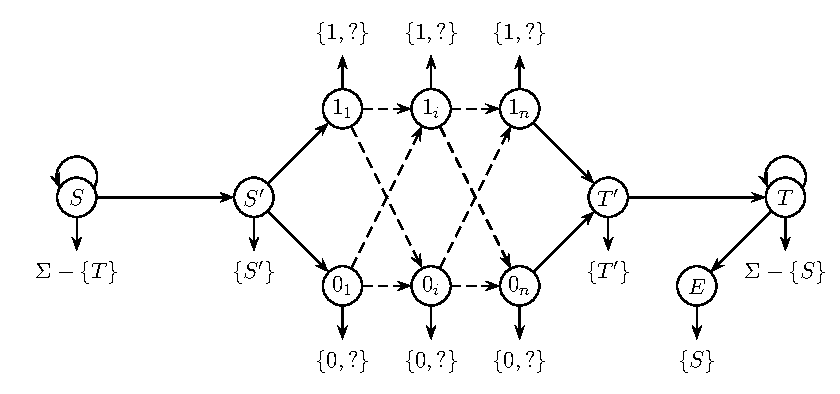
\includegraphics[scale=0.68]{../figures/jcss/expandedcliquehmm.pdf}}
\caption[HMM for which set is NP-hard to optimize]{The HMM from the proof of Theorem
  \ref{THEOREM::NPSET}. States are shown as circles; under each we
  list the set of symbols that the state emits with non-zero
  probability. Each of these symbols is emitted with probability
  $1/k$, where $k$ is the size of the set. The HMM always starts in
  state $S$. All outgoing transitions from a particular state have
  the same probability.}\label{fig:set_hmm2}
\end{figure*}

\begin{comment}
\begin{figure*}
\centerline{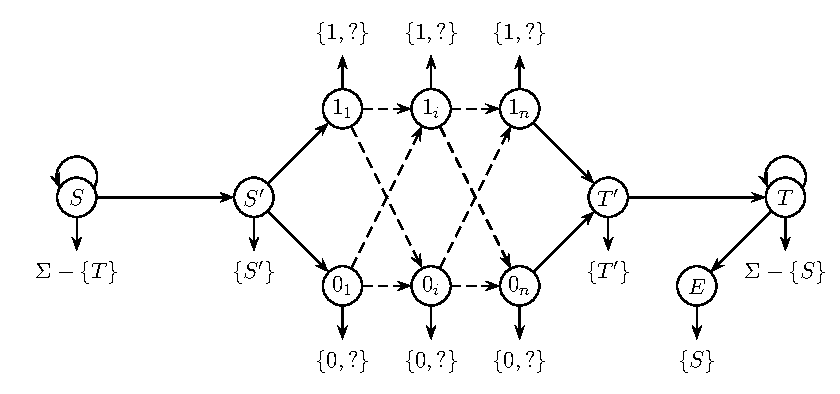
\includegraphics[scale=0.68]{../figures/jcss/expandedcliquehmm.pdf}}
\caption{The HMM from the proof of Theorem
  \ref{THEOREM::NPSET}. States are shown as circles; under each we
  list the set of symbols that the state emits with non-zero
  probability. Each of these symbols is emitted with probability
  $1/k$, where $k$ is the size of the set. The HMM always starts in
  state $S$. All outgoing transitions from a particular state have
  the same probability.}\label{fig:set_hmm2}
\end{figure*}

\begin{theorem}The following problem is NP-hard:
Given an HMM $H$, sequence $X$ of length $n$, and a number $p\in [0,1]$,
decide if there exists a set of states $S$ such that 
$\Pr\left(s(\pi)=S, X\mid H, n \right)\geq p$.
\end{theorem}\label{thm:sets}
\end{comment}
\begin{proof}
Let $G=(V,E)$ be an undirected graph with $n$ vertices as in proof of theorem
\ref{THEOREM::NPFOOT}. Note that $V = \{1, 2, \dots, n\}$. $G$ will be encoded in
sequence $X$ as in proof if theorem \ref{THEOREM::NPFOOT}, but without $\#$ symbols.
Let $X_i$ be the block that represents vertex $i$. Then $X=SX_1\dots X_nT$.

Instead of using one fixed HMM, we expand middle part of the model so that it
generates blocks of length $n+2$ ($n$ vertices and $S', T'$ states). We remove
state $\#$ and expand states $0$ and $1$ into $n$ versions of state $0$ and $1$
denoted $0_v$ and $1_v$ for $v \in V$.  Transitions are from $S'$ to $0_1$ and
$1_1$, from $0_n$ and $1_n$ to $T'$ and for all $i<n$ from $c_i$ to $d_{i+1}$
for $c,d\in \{0, 1\}$ as in figure  \ref{fig:set_hmm2}. 


State paths that generate $X$ have a similar structure as in proof of theorem
\ref{THEOREM::NPFOOT}. State $S$ generate the first symbol $S$, some initial blocks,
then one block $X_i$ is generated by some of the states $S', T', 0_v, 1_v, v\in
V$.  Rest of the sequence is generated by terminal state $T$.  Construction of
HMM and sequence $X$ guarantees that for all $v\in V$ exactly one of $0_v, 1_v$
is in the state path. Note that the set of states that is used in such state
path have exactly $n+4$ elements. We say that a state path with this structure
\emph{covers} block $X_i$. All state paths that can generate $X$ have the same
probability $q = \Pr(\pi, X\mid H, |X|) = 2^{-n^2-3n+1}6^{-n^2 - n}$.

We say that a state path $\pi$ is a \emph{run} of set $D$, if $\pi$ can generate
$X$ and $s(\pi) = D$. The probability of set $D$ is $qk$, where $k$ is the
number of runs of $D$. Every run of $S$ covers a different block, since once the
block is known, the path is uniquely determined.

We will now prove that the graph $G$ has a clique of size at least $k$ if and
only if there is a set of states for sequence $X$ with probability at least
$qk$.  First, let $R$ be a clique in $G$ of size at least $k>0$.  Consider the
set $D=\left\{S,S',{c_1},{c_2},\dots,{c_n},T',T\right\}$ where $c_i=1_i$ if
$i\in R$ and $c_i=0_i$ otherwise. For any $i\in R$, there is a run $\pi_i$ of
$D$ that covers $X_i$. This run will use state $1_j$ for generating each
$b_{i,j}$ such that $j\in R$ and thus both $b_{i,j}\in \{?,1\}$ and $c_j=1_j$.
For $j\notin R$ we have $b_{i,j}=0$ and $c_j=0_j$, thus they will use state
$0_j$ in $\pi$. Since there is a different run for every $i\in R$, set $D$ has
at least $k$ runs.

Conversely, let $D$ be a set of states with probability at least $qk>0$
and thus with at least $k$ runs. We will construct a clique of size at least $k$
as follows. Let $R$ be the set of all vertices $i$ such that $D$ has a run that
covers $X_i$. Clearly the size of $R$ is at least $k$.  Since $D$ has non-zero
probability, it has the form $\left\{S,S',c_1,c_2,\dots,c_n,T',T\right\}$ for
$c_i\in \{0_i,1_i\}$. For all $i\in R$, $c_i=1_i$ because the $i$-th block has
$b_{i,i}=1$. Therefore for all $i,j\in R$, we have $b_{i,j}\in \{1,?\}$, which
means that $(i,j)\in E$ or $i=j$. This implies that $R$ is indeed a clique.

Given graph $G$ and threshold $k$, we can compute in
polynomial time sequence $X$ and threshold $qk$ such that $G$ has a
clique of size at least $k$ if and only if sequence $X$ has a
set of states with probability at least $qk$. This completes our reduction.\qed
\end{proof}
\begin{comment}
\section{Decoding of Pair-HMM}

\notmytext{
Tu treba aj nejake veci podokazovat}
\reformulate{Tu treba aj nejake veci podokazovat}
\begin{reformulate*}
Tento text by sa mal asi reformulovat
\end{reformulate*}

\begin{notmytext*}
Intuitivne: Ked sa pohnem k parovym, tak vsetko ostane aspon rovnako tazke, ale mozno budem vediet znizit pocet stavov.
Pravdepodobne intuitivne budem vediet prekladat do znizenia poctu stavov -- v
druhej sekvencii by som mohol nejako kodovat stavy HMM s tym, ze by bola mozno
iba ciastocne vacsia
\end{notmytext*}
\end{comment}
